%-------------------------------------------------------------------------------
%-------------------------------------------------------------------------------
%-------------------------------------------------------------------------------
\chapter{Arbres binaires de recherche}
%-------------------------------------------------------------------------------
%-------------------------------------------------------------------------------
%-------------------------------------------------------------------------------
\section{Introduction}
%-------------------------------------------------------------------------------
%-------------------------------------------------------------------------------

Nous allons, dans ce chapitre, utiliser les arbres binaires ; leur principal intérêt est que chaque nœud est accessible par un chemin de longueur $h$ au plus depuis la racine  où $h$ est la hauteur de l'arbre. De plus la hauteur peut être aussi petite que $\log_2(n)$ où $n$ est la taille de l'arbre (le nombre de nœuds).

\medskip

Il reste alors deux étapes pour utiliser pleinement cette caractéristique.
%-------------------------------------------------------------------------------
\begin{itemize}
\item Comment savoir où chercher dans l'arbre ?

Il faudra ajouter une propriété supplémentaire, c'est l'objet de ce chapitre.

\item Comment assurer une hauteur qui reste de l'ordre de $\log_2(n)$ ?

Il faudra maintenir des arbres équilibrés : arbres AVL, arbres rouge-noir, arbres 2-3, \dots

Ce sera l'objet d'un T.P.
\end{itemize}
%-------------------------------------------------------------------------------------------------------------------------
%-------------------------------------------------------------------------------------------------------------------------
\subsection{Comparaisons}
%-------------------------------------------------------------------------------
%-------------------------------------------------------------------------------
On a besoin de comparer les éléments entre eux, c'est possible pour une valeur de type entier, réel ou chaîne de caractères. Pour pouvoir utiliser d'autres types de données, on utilisera une fonction \type{cle} qui associe un entier (ou un autre type muni d'une relation d'ordre) à chaque valeur de nœud : @cle 'a  -> int@.

On imposera que les clés doivent être distinctes dans l'arbre ; autrement dit la restriction de la fonction \type{cle} aux valeurs de l'arbre doit être injective.

Dans la partie {\bf 2}, les valeurs seront entières et on peut écrire @let cle x = x;;@

Dans la partie {\bf 3}, on utilisera les arbres binaires pour implémenter des dictionnaires, les valeurs des nœuds sont alors des couples clé-valeur et on peut écrire @let cle = fst;;@
%-------------------------------------------------------------------------------
%-------------------------------------------------------------------------------
\subsection{Définition}
%-------------------------------------------------------------------------------
%-------------------------------------------------------------------------------
\begin{defin}{Arbre binaire de recherche (ABR)}{abr}
Un arbre binaire de recherche est un arbre binaire tel que,  pour tout nœud $x$,  les clés des éléments du fils gauche sont strictement inférieures à la clé de $x$ et les clés des éléments du fils droit sont strictement supérieures à la clé de $x$.
\end{defin}
%-------------------------------------------------------------------------------

\begin{figure*}[h]
\centering
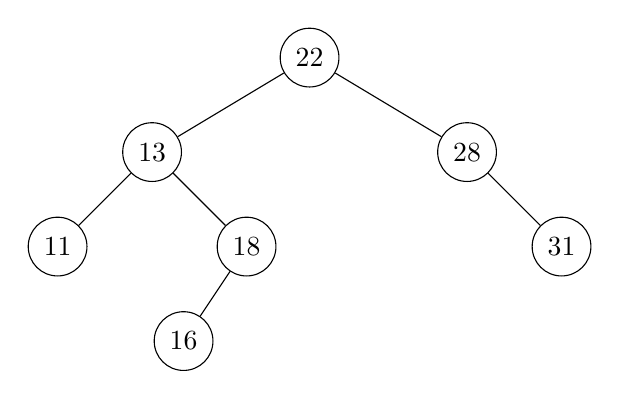
\begin{tikzpicture}[level distance =15mm,scale=0.8]
  \tikzstyle{level 1}=[sibling distance =5cm]
  \tikzstyle{level 2}=[sibling distance =3 cm]
  \tikzstyle{level 3}=[sibling distance =2 cm]
  \tikzstyle{every node}=[circle,draw]
  \node  {$22$}
  child {node{$13$}
          child {node{$11$}}
          child {node{$18$}
                  child {node{$16$}}
                  child [fill=none] {edge from parent[draw=none]}
                 }
        }
  child {node {$28$}
         child [fill=none] {edge from parent[draw=none]}
         child {node{$31$}}
        };
\end{tikzpicture}
\caption{Exemple : arbre $a_0$}
\label{g:a0}
\end{figure*}

La déclaration du type est la même que dans le cas d'un arbre binaire classique. Il faut vérifier soi--même que les clés sont distinctes et dans le bon ordre.

%-------------------------------------------------------------------------------
\begin{ocaml}
type 'a abr = Vide | Noeud of ('a abr * 'a * 'a abr);; 
\end{ocaml} 
%-------------------------------------------------------------------------------
On étudiera des arbres de type \type{int} dans les illustrations du cours.

On ne dessinera en général pas les feuilles vides.
%-------------------------------------------------------------------------------
%-------------------------------------------------------------------------------
\subsection{Exercices}
%-------------------------------------------------------------------------------
%-------------------------------------------------------------------------------
\begin{exo}{Une caractérisation}{}
Prouver qu'un arbre binaire est un arbre binaire de recherche si et seulement si le parcours {\bf infixe} des clés de l'arbre donne une suite strictement croissante.
%-------------------------------------------------------------------------------
\reponse
%-------------------------------------------------------------------------------
{\bf Sens inverse}

On suppose que le parcours infixe lit les clés dans l'ordre croissant

Pour tout sous--arbre les clés du fils gauche sont lues par le parcours infixe avant la clé de la racine donc, comme le parcours est croissant, les clés du fils gauche sont inférieures à celle de la racine. 

De même les clés du fils droit sont supérieures à celle de la racine.

L'arbre est donc bien un A.B.R.

{\bf Sens direct}


On vérifie la réciproque par récurrence sur la hauteur.

\begin{itemize}
\item C'est évident pour un sous--arbre de hauteur 0.

\item Si c'est vrai pour tous les arbres de hauteur $p$ au plus.
Les  fils droit et gauche  d'un arbre de hauteur $p+1$ ont une hauteur inférieure ou égale à $p$. Le parcours infixe de $T$ se fait en parcourant le fils gauche, qui donne des clés croissantes par hypothèse de récurrence, puis en lisant la clé de la racine, supérieure aux précédentes, puis en parcourant le fils droit, toujours en croissant.
Le parcours infixe est croissant.

\end{itemize}
\end{exo}
%-------------------------------------------------------------------------------
%-------------------------------------------------------------------------------
\begin{exo}{Rappel : parcours infixe}{}
Écrire une fonction de complexité linéaire qui renvoie  les éléments d'un arbre binaire de recherche dans une liste croissante.
%-------------------------------------------------------------------------------
\reponse
%-------------------------------------------------------------------------------
Il faut éviter d'utiliser la concaténation des listes qui donnera une complexité en $n\ln(n)$, voire en $n^2$ si l'arbre n'est pas équilibré. On va donc utiliser une fonction auxiliaire qui accumule les valeurs des nœuds à une liste passée en paramètre. On devra alors commencer par le fils droit.
\begin{ocaml}
let liste_of_arbre arbre =
  let rec aux a vu =
      match a with
      |Vide -> vu
      |Noeud(g, r, d) -> aux g (r::(aux d vu))
  in aux arbre [];;
\end{ocaml}
\end{exo}
%-------------------------------------------------------------------------------
%-------------------------------------------------------------------------------
\begin{exo}{Vérification}{}

Écrire une fonction qui teste si l'arbre binaire passé en paramètre est un arbre binaire de recherche.
%-------------------------------------------------------------------------------
\reponse
%-------------------------------------------------------------------------------
\type{Noeud(g, r, d)} est un arbre binaire de recherche si 

 \type{g} et \type{d} sont des arbres binaires de recherche,

 le maximum des clés de \type{g} est strictement inférieur à $n$,
 
 le minimum des clés de \type{d} est strictement supérieur à $n$.
 
 On peut calculer les maximums et minimums par des fonctions auxiliaire mais cela revient à parcourir tout l'arbre plusieurs fois. On va tout calculer d'un coup.
 
L'arbre vide n'a pas de maximum, on le remplace par l'entier minimum : tout entier lui sera supérieur. De même le minimum de l'arbre vide sera choisi comme l'entier maximum.
%-------------------------------------------------------------------------------
\begin{ocaml}
let estABR arbre = 
  let rec aux a =
      match a with
      |Vide -> (max_int, true, min_int)
      |Noeud(g, r, d) -> let (min1, b1, max1) = aux g in 
                         let (min2, b2, max2) = aux d in
                         let k = cle r in
                         (min1, 
                          b1 && b2 && (max1 < k) && (k < min2), 
                          max2)
  in let (_,b,_) = aux arbre in b;;
\end{ocaml}

On peut aussi choisir de traiter à part le cas de l'arbre vide et de séparer les nœuds selon le nombre de fils vides.
%-------------------------------------------------------------------------------
\begin{ocaml}
let estABR arbre = 
  let rec aux a =
      match a with
      |Vide -> (0, true, 0)
      |Noeud(Vide, r, Vide) -> let k = cle r in (k, true, k)
      |Noeud(Vide, r, d) ->  let (min2, b2, max2) = aux d in
                             let k = cle r in
                             (k, b2 && (k < min2), max2)
      |Noeud(g, r, Vide) -> let (min1, b1, max1) = aux g in 
                            let k = cle r in
                            (min1, b1 && (max1 < k), k)
      |Noeud(g, r, d) -> let (min1, b1, max1) = aux g in 
                         let (min2, b2, max2) = aux d in
                         let k = cle r in
                         (min1, 
                          b1 && b2 && (max1 < k) && (k < min2), 
                          max2)
  in let (_,b,_) = aux arbre in b;;
\end{ocaml}
\end{exo}
%-------------------------------------------------------------------------------
%-------------------------------------------------------------------------------
\begin{exo}{Préfixes d’un arbre binaire}{}

On dit qu’un arbre binaire {\tt t} est un préfixe d’un arbre binaire {\tt t1} si {\tt t} est l’arbre vide ou si {\tt t = Noeud(g,k,d)} et {\tt t1 = Noeud(g1,k,d1)} avec {\tt g} prefixe de {\tt g1} et {\tt d} prefixe de {\tt d1}.

\begin{itemize}
\item Montrer que la relation {\it "est prefixe de"} est un ordre partiel sur les arbres binaires.

\item Montrer que tout préfixe d’un ABR est un ABR.

\item Écrire une fonction testant si un arbre binaire est préfixe d’un autre.
\end{itemize}
%-------------------------------------------------------------------------------
\reponse
%-------------------------------------------------------------------------------
\begin{itemize}
\item Réflexivité et transitivité sont immédiates.

La symétrie peut se prouver par récurrence sur la taille ou sur la hauteur.

\item Par récurrence sur la taille ou sur la hauteur ou par induction structurelle.

\item 
\begin{ocaml}
let rec est_prefixe a1 a2 =
  match a1, a2 with
  |Vide, _ -> true
  |Noeud(g1, r1, d1), Noeud(g2, r2, d2) when r1 = r2
      -> (est_prefixe g1 g2) && (est_prefixe d1 d2)
  |_ -> false;;
\end{ocaml}
\end{itemize}
\end{exo}
%-------------------------------------------------------------------------------
%-------------------------------------------------------------------------------
\section{Recherche}
%-------------------------------------------------------------------------------
%-------------------------------------------------------------------------------
\subsection{Algorithme}
%-------------------------------------------------------------------------------
%-------------------------------------------------------------------------------
Une fonction de base est la recherche d'un élément dans un arbre : on renvoie un booléen indiquant s'il existe un élément de clé donnée dans l'arbre. Pour cela on ''descend'' dans l'arbre en choisissant le fils gauche ou le fils droit selon que la valeur à chercher est inférieure ou supérieure au la clé de la racine. On remarque que c'est le principe de la recherche par dichotomie

On parcourt ainsi (partiellement) une branche de l'arbre.

\medskip

Si on aboutit à la valeur, c'est qu'elle est dans l'arbre. 

\begin{figure*}[h]
\centering
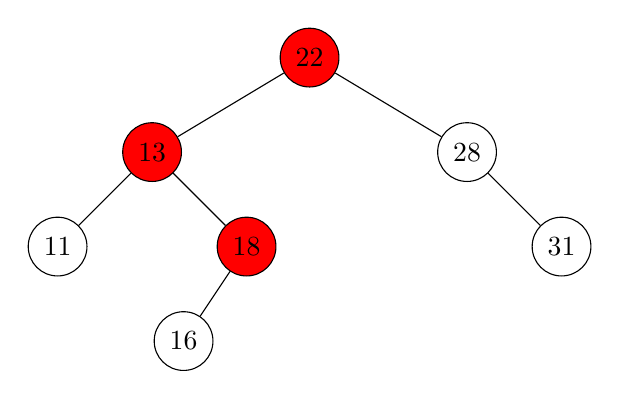
\begin{tikzpicture}[level distance =15mm,scale=0.8]
  \tikzstyle{level 1}=[sibling distance =5cm]
  \tikzstyle{level 2}=[sibling distance =3 cm]
  \tikzstyle{level 3}=[sibling distance =2 cm]
  \tikzstyle{every node}=[circle,draw]
  \node[fill=red] {$22$}
  child {node[fill=red]{$13$}
          child {node{$11$}}
          child {node[fill=red]{$18$}
                  child {node{$16$}}
                  child [fill=none] {edge from parent[draw=none]}
                 }
        }
  child {node{$28$}
         child [fill=none] {edge from parent[draw=none]}
         child {node{$31$}}
        };
\end{tikzpicture}
\caption{Recherche de 18 dans l'arbre $a_0$}
\end{figure*}

Par contre, si on aboutit à une feuille, c'est que la valeur n'est pas dans l'arbre. 

\begin{figure*}[h]
\centering
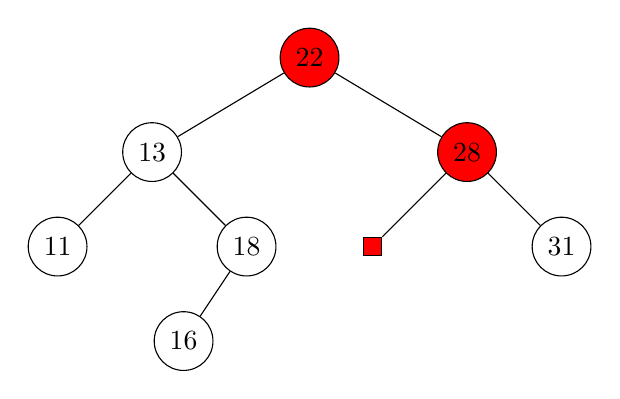
\begin{tikzpicture}[level distance =15mm,scale=0.8]
  \tikzstyle{level 1}=[sibling distance =5cm]
  \tikzstyle{level 2}=[sibling distance =3 cm]
  \tikzstyle{level 3}=[sibling distance =2 cm]
  \tikzstyle{every node}=[circle,draw]
  \node[fill=red] {$22$}
  child {node{$13$}
          child {node{$11$}}
          child {node{$18$}
                  child {node{$16$}}
                  child [fill=none] {edge from parent[draw=none]}
                 }
        }
  child {node[fill=red]{$28$}
         child {node[rectangle, draw, fill=red] {}}
         child {node{$31$}}
        };
\end{tikzpicture}
\caption{Recherche de 23 dans l'arbre $a_0$}
\end{figure*}
%-------------------------------------------------------------------------------
\begin{code}{Recherche dans un arbre binaire de recherche}
let rec chercher k arbre = 
  match arbre with
  |Vide -> false
  |Noeud(g, r, d) when cle r = k -> true
  |Noeud(g, r, d) when k < cle r -> chercher k g
  |Noeud(g, r, d) -> chercher k d;;
\end{code}
%-------------------------------------------------------------------------------
%-------------------------------------------------------------------------------
\subsection{Analyse}
%-------------------------------------------------------------------------------
%-------------------------------------------------------------------------------
Nous allons établir la terminaison, la preuve et la complexité en même temps en séparant les cas où la clé recherchée est ou n'est pas dans l'arbre.  La complexité est comptée en nombre de comparaisons.
%-------------------------------------------------------------------------------
\subsubsection{Absence de la clé}
%-------------------------------------------------------------------------------
 Si la clé n'est pas dans l'arbre, chaque appel de la fonction à partir d'un sous-arbre non vide fera un appel à la fonction avec un des deux fils. Ainsi la hauteur de l'arbre en paramètre de la fonction diminue strictement à chaque appel. Comme la hauteur ne peut être inférieure à -1 le nombre d'appel est fini et on aboutit à un appel \type{chercher x Vide} qui renvoie \type{false}.
 
L'algorithme termine en renvoyant la bonne réponse. De plus la diminution  d'au moins 1 de la hauteur à chaque appel récursif montre que le nombre d'appel est au plus $h+1$. Comme on fait 2 comparaisons à chaque appel sauf pour le cas de l'arbre vide la complexité en nombre de comparaisons est majorée par $2(h+1)$ ($h$ est la hauteur de l'arbre).
\newpage
%-------------------------------------------------------------------------------
\subsubsection{Clé présente}
%-------------------------------------------------------------------------------
 En s'inspirant du résultat ci-dessus on note ${\cal P}_h$ la propriété :
\poser{${\cal P}_h$}
{Pour tout arbre \type{a} de hauteur $h$ et pour toute clé \type{k} apparaissant dans l'arbre 
\type{chercher k a} renvoie \type{true} avec $2h+1$ comparaisons au plus.}

On notera que l'arbre est non vide car il contient au moins le nœud de clé $k$, ainsi $h\ge 0$.

\begin{description}
\item[Initialisation] ${\cal P}_0$ est vraie car un arbre de hauteur 0 qui au moins une clé ne peut être qu'un arbre de la forme 
\type{Noeud(Vide, r,  Vide)}  avec \type{cle x = k} :  dans ce cas la fonction renvoie \type{true} après 1 comparaison.

\item[Progression] On suppose que  ${\cal P}_m$ est vraie pour tout $m< h$ ($h\ge 1$). 

\type{a = Noeud(g, r, d)} est un arbre de hauteur $h$ qui contient  un élément de clé \type{k}.

\begin{itemize}
\item Si on a \type{cle r = k}, la fonction \type{chercher k a} renvoie \type{true} avec 1 comparaison.

\item Si on a \type{k <cle r} alors l'élément de clé $k$ ne peut pas être \type{d} donc \type{g} contient \type{k} et est de hauteur $h-1$ au plus.

 \type{chercher k a} effectue 2 comparaisons puis appelle \type{chercher k g} qui, d'après l'hypothèse de récurrence, renvoie \type{true} après $2(h-1)+1$ comparaisons au plus. 
 
 Ainsi \type{chercher k a} renvoie \type{true} avec $2h-1+2$ comparaisons au plus.
 
\item De même si on a \type{cle r < k} alors \type{d} contient la clé \type{k}  et \type{chercher k a} renvoie \type{true} avec $2h-1+2$ comparaisons au plus.
\end{itemize}
\item[Conclusion] La propriété est prouvée par récurrence.

\end{description}

 On a ainsi prouvé que l'algorithme termine dans tous les cas, qu'il renvoie la réponse exacte et que la complexité est majorée par $2h+2$, c'est un ${\cal O}(h)$.
%-------------------------------------------------------------------------------
%-------------------------------------------------------------------------------
\subsection{Valeur du nœud}
%-------------------------------------------------------------------------------
%-------------------------------------------------------------------------------
Si un élément de clé $k$ existe, la recherche ci-dessus parvient au nœud dont la clé est $k$. On peut transformar la fonction pour qu'elle renvoie sa valeur.
%-------------------------------------------------------------------------------
\begin{code}{Valeur d'un nœud en fonction de sa clé}
let rec noeud k arbre = 
  match arbre with
  |Vide -> failwith "L'arbre ne contient pas la clé"
  |Noeud(g, r, d) when cle r = k -> r
  |Noeud(g, r, d) when k < cle r -> noeud k g
  |Noeud(g, r, d) -> noeud k d;;
\end{code}
%-------------------------------------------------------------------------------
%-------------------------------------------------------------------------------
\subsection{Exercices}
%-------------------------------------------------------------------------------
%-------------------------------------------------------------------------------
\begin{exo}{Parcours de recherche}{}

On suppose que tous les nombres de 1 à 800 sont les clés d'un 
arbre binaire de recherche. Parmi les suites suivantes lesquelles ne peuvent pas être les clés d'un parcours de recherche de 417 ?

\begin{itemize}

\item 222, 457, 122, 217, 417

\item 601, 403, 555, 408, 523, 411, 466, 417

\item 601, 403, 555, 408, 563, 411, 466, 417

\item 901, 403, 555, 411, 466, 417
\end{itemize}
%-------------------------------------------------------------------------------
\reponse
%-------------------------------------------------------------------------------
Le principe est que si on suit un arbre binaire de recherche $u_0, u_1, \ldots, u_p$ $u_{i+1} > u_i$ impose $u_j > u_i$ pour tout $j>i$.


\begin{itemize}
\item 122 n'est pas possible après 222, 457

\item 545, 215, 333, 401, 422, 417 est possible 


\item 601, 403, 555, 408, 523, 411, 466, 417 est possible


\item 563 n'est pas possible après 601, 403, 555, 408


\item 901, 403, 555, 411, 466, 417 est possible
\end{itemize}
\end{exo}
%-------------------------------------------------------------------------------
%-------------------------------------------------------------------------------
\begin{exo}{Tranche}{}
Écrire une fonction \type{tranche arbre a b} qui reçoit comme paramètre un arbre binaire de recherche et deux entiers et qui renvoie un arbre binaire de recherche dont les nœuds sont les nœuds de l'arbre initial qui leur clé  comprise entre \type{a} et \type{b}.
%-------------------------------------------------------------------------------
\reponse
%-------------------------------------------------------------------------------
\begin{ocaml}
let rec tranche arbre a b = 
  match arbre with
  |Vide -> Vide
  |Noeud(g, r, d) when cle r < a -> tranche d a b
  |Noeud(g, r, d) when cle r > b -> tranche g a b
  |Noeud(g, r, d) -> Noeud(tranche g a b, r, tranche d a b);;
\end{ocaml}
\end{exo}
%-------------------------------------------------------------------------------
%-------------------------------------------------------------------------------
\section{Insertion}
%-------------------------------------------------------------------------------
%-------------------------------------------------------------------------------
\subsection{Insertion aux feuilles}
%-------------------------------------------------------------------------------
Lorsque l'on cherche un élément qui n'est pas dans l'arbre, on aboutit à une feuille ; on peut alors remplacer la feuille par un nœud terminal.

Si l'élément était déjà présent, on ne change rien.

\medskip

Ici encore la complexité est proportionnelle au nombre d'appels récursifs effectués donc est de la forme ${\cal O}(h)$ où $h$ est la hauteur de l'arbre.

{\bf Exemple} : on ajoute 25 à l'exemple initial :

\begin{figure*}[h]
\centering
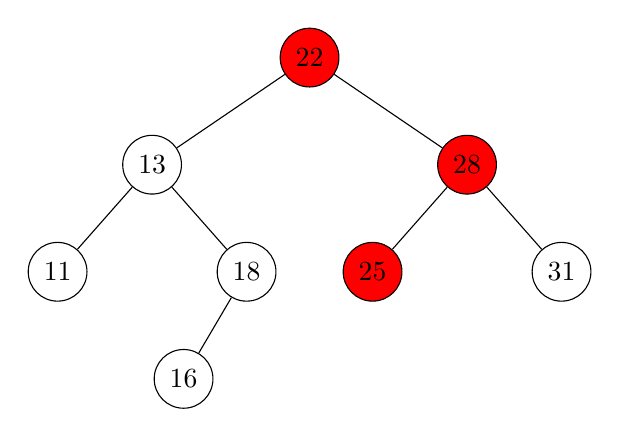
\begin{tikzpicture}[level distance =17mm,scale=0.8]
  \tikzstyle{level 1}=[sibling distance =5cm]
  \tikzstyle{level 2}=[sibling distance =3 cm]
  \tikzstyle{level 3}=[sibling distance =2 cm]
  \tikzstyle{every node}=[circle,draw]
  \node[fill=red] {$22$}
  child {node{$13$}
          child {node{$11$}}
          child {node{$18$}
                  child {node{$16$}}
                  child [fill=none] {edge from parent[draw=none]}
                 }
        }
  child {node[fill=red]{$28$}
              child {node[fill=red]{$25$}}
              child {node{$31$}}
        };
\end{tikzpicture}
\caption{Ajout de 25 dans une feuille de l'arbre $a_0$.}
\end{figure*}
%-------------------------------------------------------------------------------
\begin{code}{Insertion aux feuilles}
let rec insertionF x arbre = 
  match arbre with
  |Vide -> Noeud(Vide, x,  Vide)
  |Noeud(g, r d) when cle r = cle x-> Noeud(g, x, d)
  |Noeud(g, r, d) when cle x = cle r
                  -> Noeud((insertionF x  g), r, d)
  |Noeud(g, r, d) -> Noeud(g, r, (insertionF x  d));;
\end{code}
%-------------------------------------------------------------------------------
%-------------------------------------------------------------------------------
\subsection{Insertion à la racine}
%-------------------------------------------------------------------------------
On peut aussi choisir d'insérer un nouveau nœud en le plaçant à la racine.

Pour cela on va couper l'arbre en deux parties regroupant les nœuds inférieurs à la nouvelle clé et ceux qui sont supérieurs.

La première étape consiste à produire les deux arbres séparés par la clé de l'élément que l'on veut ajouter. Le découpage et la reconstitution se font en même temps, récursivement.

Si la clé de la valeur est strictement inférieure à celle de la racine, on découpe le fils gauche avec la clé de la valeur à ajouter.

On obtient deux arbres : \type{g\_inf}, l'arbre formés des nœuds du fils gauche de clé inférieure à la coupure et, symétriquement, \type{g\_sup}.

L'arbre des nœuds inférieurs à la coupure est alors \type{g\_inf} et l'arbre des nœuds supérieurs à la coupure est formé en remplaçant le fils gauche initial par \type{g\_sup}.

On fait les opérations symétriques si la coupure est strictement supérieure à la racine.

En cas d'égalité on retire la racine et on renvoie les deux fils. 
%-------------------------------------------------------------------------------
\begin{code}{Insertion à la racine}
let rec decoupage k a = 
  match a with
  |Vide -> (Vide,Vide)
  |Noeud(g, r, d) when cle r = k -> (g, d)
  |Noeud(g, r, d) when k < cle r
                  -> let (gg, gd) = decoupage k g 
                      in (gg, Noeud(gd, r, d))
  |Noeud(g, r, d) -> let (dg, dd) = decoupage k d 
                      in (Noeud(g, r, dg),dd);;
                
let insertionRacine x a =
  let (g, d)= decoupage (cle x) a 
  in Noeud(g,x, d);;
\end{code}
%-------------------------------------------------------------------------------
Ici encore on remplace l'élément de l'arbre qui a une clé égale à celle de l'élément à ajouter.
%-------------------------------------------------------------------------------
\begin{figure*}[h]
\centering
\begin{tikzpicture}\tikzstyle{every node}=[circle,draw,minimum size=8mm]
\node at (0,-0.2) (r) {22};
\node at (-2.5,-1.5) (fg) {13};
\node at (2.5,-1.5) (fd) {28};
\node at (-4,-2.8) (fgg) {11};
\node at (-1,-2.8) (fgd) {18};
\node at (4,-2.8) (fdd) {31};
\node at (-2,-4) (fgdg) {16};
\draw (r) -- (fd)
     (fg) -- (fgg)
     (fd) -- (fdd);
\draw [red,dashed]
      (r) -- (fg)
     (fg) -- (fgd)
    (fgd) -- (fgdg);
\draw[>-<,thick, red] (-1.5, 0.5) --  (-1.5,-5);
\end{tikzpicture}
\caption{Séparation de l'arbre $a_0$ par la clé 17}
%-------------------------------------------------------------------------------
\bigskip
%-------------------------------------------------------------------------------
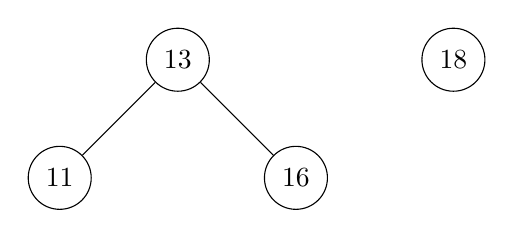
\begin{tikzpicture}
\tikzstyle{every node}=[circle,draw,minimum size=8mm]
\node at (-5,0) (fg) {13};
\node at (-6.5,-1.5) (fgg) {11};
\node at (-1.5,0) (fgd) {18};
\node at (-3.5,-1.5) (fgdg) {16};
\draw (fg) -- (fgg)
      (fg) -- (fgdg);
\end{tikzpicture}
\caption{Reconstitution du fils gauche}
\end{figure*}
%-------------------------------------------------------------------------------
\clearpage
\newpage
%-------------------------------------------------------------------------------
\begin{figure*}[h]
\centering
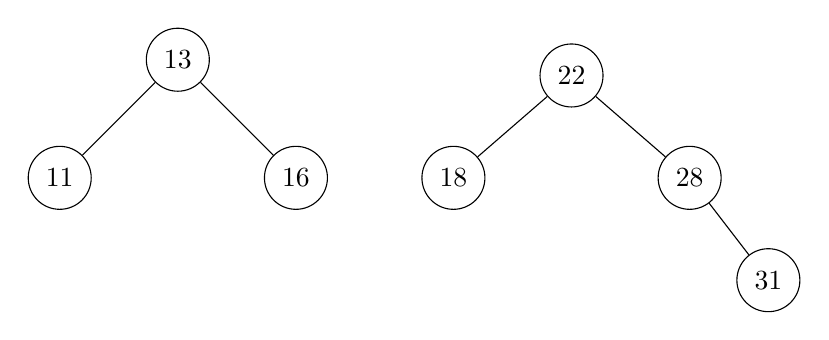
\begin{tikzpicture}\tikzstyle{every node}=[circle,draw,minimum size=8mm]
\node at (0,-0.2) (r) {22};
\node at (-5,0) (fg) {13};
\node at (1.5,-1.5) (fd) {28};
\node at (-6.5,-1.5) (fgg) {11};
\node at (-1.5,-1.5) (fgd) {18};
\node at (2.5,-2.8) (fdd) {31};
\node at (-3.5,-1.5) (fgdg) {16};
\draw (r) -- (fd)
      (r) -- (fgd)
     (fg) -- (fgg)
     (fg) -- (fgdg)
     (fd) -- (fdd);
\end{tikzpicture}
\caption{Reconstruction des deux arbres.}
%-------------------------------------------------------------------------------
\bigskip
%-------------------------------------------------------------------------------
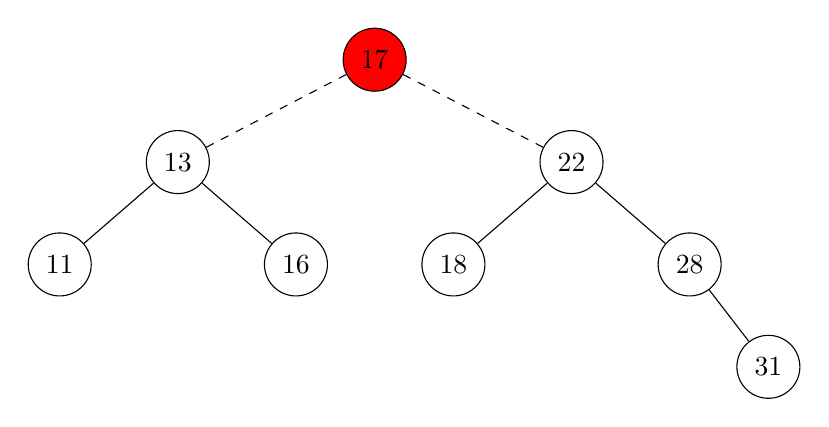
\begin{tikzpicture}\tikzstyle{every node}=[circle,draw,minimum size=8mm]
\node[fill=red] at (-2.5,1.1) (r0) {17};
\node at (0,-0.2) (r) {22};
\node at (-5,-0.2) (fg) {13};
\node at (1.5,-1.5) (fd) {28};
\node at (-6.5,-1.5) (fgg) {11};
\node at (-1.5,-1.5) (fgd) {18};
\node at (2.5,-2.8) (fdd) {31};
\node at (-3.5,-1.5) (fgdg) {16};
\draw (r) -- (fd)
      (r) -- (fgd)
     (fg) -- (fgg)
     (fg) -- (fgdg)
     (fd) -- (fdd);
\draw[dashed]  (r0) -- (r)
              (r0) -- (fg);
\end{tikzpicture}
\caption{Ajout de 17 à la racine.}
\end{figure*}
%-------------------------------------------------------------------------------
%-------------------------------------------------------------------------------
\subsection{Exercices}
%-------------------------------------------------------------------------------
%-------------------------------------------------------------------------------
\begin{exo}{Remplissage d'un arbre}{}
Écrire une fonction \type{arbre\_of\_liste} qui crée un arbre à partir d'une liste en ajoutant un-par-un les éléments de la liste à un arbre vide.
%-------------------------------------------------------------------------------
\reponse
%-------------------------------------------------------------------------------
\begin{ocaml}
let arbre_of_liste liste =
  let rec aux l fait =
      match l with
      |[] -> fait
      |t::q -> aux q (insertionF t fait)
  in aux liste Vide;;
\end{ocaml}
\end{exo}
%-------------------------------------------------------------------------------
%-------------------------------------------------------------------------------
\begin{exo}{Tri}{}
Comment peut-on utiliser les arbres binaires de recherche pour effectuer un tri ?

Si on admet que la hauteur moyenne d'un arbre binaire de recherche de taille $n$ est un ${\cal O}\bigl(\log_2(n)\bigr)$ déterminer la complexité, en moyenne, de ce tri.

Écrire une fonction de tri de liste utilisant cette méthode.
%-------------------------------------------------------------------------------
\reponse
%-------------------------------------------------------------------------------

L'arbre sert de réservoir qui trie tout seul les éléments qu'on lui ajoute.

\begin{itemize}
\item On insère (dans le désordre) les éléments à trier dans un arbre à partir de l'arbre vide.

\item On lit l'arbre dans un parcours infixe : la liste est triée.

\end{itemize}

La complexité des insertions est de l'ordre de $\displaystyle \sum_{i=1}^{n-1} \ln(i)\le n\log_2(n)$.

Le parcours est de complexité linéaire donc le tri est un ${\cal O}\bigl(n\log_2(n)\bigr)$.

\begin{ocaml}
let tri_ABR liste =
  liste_of_arbre (arbre_of_liste liste);;
\end{ocaml}
\end{exo}
%-------------------------------------------------------------------------------
%-------------------------------------------------------------------------------
\begin{exo}{Nombre de constructions}{}

Déterminer tous les ordres possibles d'insertion de clés à partir de l'arbre vide qui donnent l'arbre suivant par adjonction aux feuilles

\begin{center}
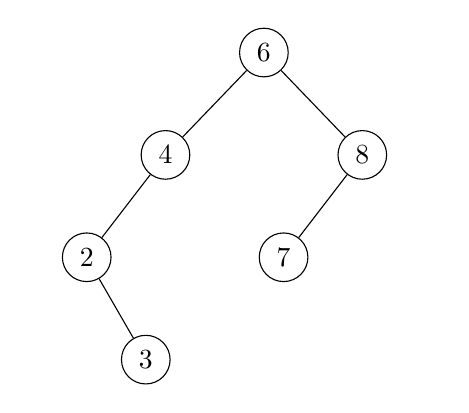
\begin{tikzpicture}
  \tikzstyle{level 1}=[level distance =13 mm,sibling distance =25 mm]
  \tikzstyle{level 2}=[level distance =13 mm,sibling distance =20 mm]
  \tikzstyle{level 3}=[level distance =13 mm,sibling distance =15 mm]
  \tikzstyle{every node}=[circle,draw]
  \node {$6$}
  child {node{$4$}
          child {node{$2$}
                  child [fill=none] {edge from parent[draw=none]}
                  child {node{$3$}}
                 }
          child [fill=none] {edge from parent[draw=none]}
        }
  child {node{$8$}
          child {node{$7$}}
          child [fill=none] {edge from parent[draw=none]}
         }
  ;
\end{tikzpicture}\end{center}


Plus généralement montrer que le nombre de permutations des clés d'un arbre $T$, de taille $n$, qui engendrent l'arbre par adjonctions successives aux feuilles est $n!$ divisé par le produit des tailles de tous les sous--arbres (y compris $T$) de $T$.
%-------------------------------------------------------------------------------
\reponse
%-------------------------------------------------------------------------------
Les ordres d'insertions possibles sont :
6, 4, 2, 3, 8, 7

6, 4, 2, 8, 3, 7

6, 4, 2, 8, 7, 3

6, 4, 8, 2, 3, 7

6, 4, 8, 2, 7, 3

6, 4, 8, 7, 2, 3

6, 8, 4, 2, 3, 7

6, 8, 4, 2, 7, 3

6, 8, 4, 7, 2, 3

6, 8, 7, 4, 2, 3

\medskip

On prouve la propriété par récurrence sur la taille $n$.

La propriété est simple pour $n=1$ : il y a une seule manière de construire l'arbre.

On suppose que la propriété est vraie pour tous les arbres (non vides) de taille $k < n$.

\type{T = Noeud(g, x, s)} est un arbre de taille $n$ avec $g$ de taille $p$ et $d$ de taille $q$.

Les sous-arbres de $T$ sont les sous-arbres de $d$, les sous-arbres de $g$ et $T$.

On suppose d'abord que $g$ et $d$ sont non vides.

Pour engendrer $T$ on doit commencer par $x$ puis on doit engendrer $d$ et $g$ en choisissant un remplissage de chacun et l'ordre d'insertion des élément à droite et à gauche. 

\begin{itemize}
\item Il y a $\displaystyle \frac {p!}{\displaystyle \prod_{t\in g}|t|!}$ façon d'engendrer $g$.
\item Il y a $\displaystyle \frac {q!}{\displaystyle \prod_{t\in d}|t|!}$ façon d'engendrer $d$.
\item Pour distribuer les insertions à droite et à gauche on doit choisir les $p$ occurrences d'ajout à gauche parmi les $p+q$ : il y a donc $\displaystyle \frac {(p+q)!}{p!q!}=\frac {(n-1)!}{p!q!}$ telles distributions.
\end{itemize}

On trouve donc $\displaystyle \frac {p!}{\displaystyle \prod_{t\in g}|t|!}
\frac {q!}{\displaystyle \prod_{t\in d}|t|!}
\frac {(n-1)!}{p!q!}
=\frac {(n-1)!}{\displaystyle \prod_{t\in g}|t|!\prod_{t\in d}|t|!}
=\frac {n!}{\displaystyle |T|\prod_{t\in g}|t|!\prod_{t\in d}|t|!}
=\frac {n!}{\displaystyle \prod_{t\in T}|t|!}$.

La propriété est donc vraie pour $T$.

Si $d$ (ou $g$) est vide on construit $T$ en insérant $x$ puis les éléments de $g$ (ou $d$) : il y a le même nombre de construction et $\displaystyle \frac {(n-1)!}{\displaystyle \prod_{t\in g}|t|!}
=\frac {n!}{\displaystyle |T|\prod_{t\in g}|t|!}
=\frac {n!}{\displaystyle \prod_{t\in T}|t|!}$

La propriété est encore vraie pour $T$, c'est-à-dire pour tous les arbres de taille $n$.

On a prouvé la récurrence.
\end{exo}
%-------------------------------------------------------------------------------
%-------------------------------------------------------------------------------

\medskip
On considère les arbres binaires de recherche construits en ajoutant à l'arbre vide les nœuds de clé 1 à $n$ dans le désordre.

On suppose que les $n!$ ordres d'insertion sont équiprobables.

On cherche la complexité moyenne, en nombre de comparaisons, de la recherche d'une clé dans l'arbre : $a_n$.

On note $a_{i,n}$ la complexité moyenne, en nombre de comparaisons, de la recherche d'une clé dans un arbre dont la racine a la clé $i$.
%-------------------------------------------------------------------------------
%-------------------------------------------------------------------------------
\begin{exo}{Complexité moyenne d'une recherche}{}

\begin{itemize}
\item Prouver que $\displaystyle a_{i,n}=(a_{i-1}+2)\frac{i-1}n+\frac 1n+(a_{n-i}+2)\frac{n-i}n$.

\item En déduire que $\displaystyle a_n = 2 - \frac1n +\frac 2{n^2}\sum_{i=1}^{n-1} ia_i$

\item En calculant $n^2a_n-(n-1)^2a_{n-1}$ prouver que $\displaystyle a_n= \frac 1{n^2}\bigl((n^2-1)a_{n-1}+4n-3\bigr)$ 

\item Prouver que $a_n={\cal O}\bigl(\log_2(n)\bigr)$, {\it on pourra poser $u_n=\frac n{n+1}a_n$}.
\end{itemize}
%-------------------------------------------------------------------------------
\reponse
%-------------------------------------------------------------------------------
\begin{itemize}
\item Quand on recherche un élément de clé $k$ dans un arbre de racine $i$, 3 cas sont possible selon la valeur de $k$.

\begin{itemize}
\item Si $k=i$ on ne fait qu'une comparaison. La probabilité de $k=i$ est $\frac 1n$.
\item Si on a $k < i$ (pour $i\ge 2$) on fait deux comparaisons puis on cherche l'élément dans un arbre de taille $i-1$. La probabilité de cet événement est $\frac{i-1}n$.
\item Si on a $k > i$ (pour $i\ne n-1$) on fait deux comparaisons puis on cherche l'élément dans un arbre de taille $n-i$. La probabilité de cet événement est $\frac{n-i}n$.
\end{itemize} 

L'espérance est donc $\displaystyle \frac 1n+\frac {i-1}n(2+a_{i-1}) + \frac {n-i}n(2+a_{n-i})$.

Pour $i=1$ ou $i=n$ on trouver la valeur $\displaystyle \frac 1n+ \frac {n-1}n(2+a_{n-1})$.

\item On a $\displaystyle a_i = \sum_{i=1}^n \frac 1n a_{i,n}$ d'où, en regroupant,

\begin{align*}
a_i 
&= \sum_{i=1}^n \frac 1{n^2} 
 + \sum_{i=2}^n \frac {i-1}{n^2}(2+a_{i-1})
 + \sum_{i=1}^{n-1} \frac {n-i}{n^2}(2+a_{n-i})
\\&
 =n\frac 1{n^2} + \frac 2{n^2}\sum_{i=2}^n (i-1) + \frac 2{n^2}\sum_{i=1}^{n-1} (n-i)
 + \frac 1{n^2}\sum_{i=2}^n (i-1)a_{i-1}
 + \frac 1{n^2}\sum_{i=1}^n (n-i)a_{n-i}
\\ &
 =\frac 1n + \frac 2{n^2}\sum_{p=1}^{n-1} p +\frac 2{n^2}\sum_{p=1}^{n-1} p
 + \frac 1{n^2}\sum_{p=1}^{n-1} pa_p
 + \frac 1{n^2}\sum_{p=1}^{n-1} pa_p
\\ &
 =\frac 1n + \frac 4{n^2}\frac {n(n-1)}2
 + 2\frac 1{n^2}\sum_{p=1}^{n-1} pa_p
 = 2 -\frac 1n + \frac 2{n^2}\sum_{p=1}^{n-1} pa_p
\end{align*}

\item En utilisant l'indication proposée on obtient
\begin{align*}
n^2a_n-(n-1)^2a_{n-1}
&
=2n^2-n+2\sum_{p=1}^{n-1} pa_p
-\left(2(n-1)^2-(n-1)+2\sum_{p=1}^{n-2} pa_p\right)
\cr &
=4n-3+2(n-1)a_{n-1}\hbox{ pour }n \ge 2
\end{align*}

On obtient donc $\displaystyle a_n = \frac 1{n^2}\left(4n-3+2(n-1)a_{n-1} + (n-1)^2a_{n-1}\right)$

d'où $\displaystyle a_n = \frac 1{n^2}\left(4n-3+(n^2-1)a_{n-1}\right)$.

\item On commence par étudier les suites définies par la formule homogène 

$\displaystyle u_n = \frac 1{n^2}\left((n^2-1)u_{n-1}\right) = \frac{(n+1)(n-1)}{n^2} u_{n-1}$

Ainsi $\displaystyle u_n = \frac{(n+1) \cdots 3.(n-1)\cdots 1}{(n(n-1)\cdots 2)^2}u_1
=\frac{n+1}{2n}u_1=K\frac{n+1}n$.

On pose alors (en faisant varier la constante) $a_n = \frac{n+1}{n}b_n$.

La récurrence devient $\displaystyle \frac{n+1}{n}b_n 
= \frac 1{n^2}\left(4n-3+(n^2-1)\frac n{n-1}b_{n-1}\right)$ donc

$\displaystyle b_n = \frac{4n-3}{n(n+1)} + b_{n-1}
 = \frac 7{n+1} - \frac 3n + b_{n-1}$.
 
On a alors $\displaystyle b_n = \sum_{k=2}^n \frac 7{k+1} - \frac 3k + b_1
=\frac 7{n+1} + 4\sum_{k=1}^n \frac 1k -\frac{15}2 + b_1$.

Comme on a $b_1=\frac 12 a_1= \frac 12$ on a 
$\displaystyle a_n =\frac 7n + \frac{4(n+1)}n\sum_{k=1}^n \frac 1k -7\frac {n+1}n$.

Ainsi $\displaystyle a_n = \frac{4(n+1)}n\sum_{k=1}^n \frac 1k -7 \simeq 4\ln(n)$.
\end{itemize}
\end{exo}
%-------------------------------------------------------------------------------
%-------------------------------------------------------------------------------
\section{Suppression}
%-------------------------------------------------------------------------------
%-------------------------------------------------------------------------------
La suppression d'un nœud demande de conserver la structure ordonnée. On nommera allégé un arbre binaire de recherche obtenu en ôtant un nœud.

Il est relativement facile de supprimer un nœud terminal : on le remplace par une feuille.

Un autre cas simple est celui d'un nœud sans fils gauche (ou droit) : l'arbre allégé est obtenu en remplaçant ce nœud par son fils droit (ou gauche).

%-------------------------------------------------------------------------------
\begin{figure*}[h]
\centering
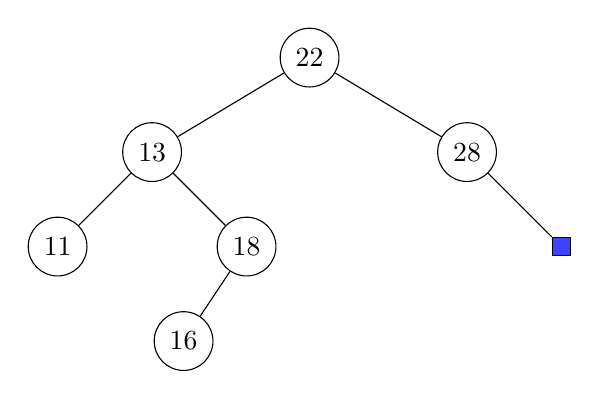
\begin{tikzpicture}[level distance =15mm,scale=0.8]
  \tikzstyle{level 1}=[sibling distance =5cm]
  \tikzstyle{level 2}=[sibling distance =3 cm]
  \tikzstyle{level 3}=[sibling distance =2 cm]
  \tikzstyle{every node}=[circle,draw]
  \node  {$22$}
  child {node{$13$}
          child {node{$11$}}
          child {node{$18$}
                  child {node{$16$}}
                  child [fill=none] {edge from parent[draw=none]}
                 }
        }
  child {node {$28$}
         child [fill=none] {edge from parent[draw=none]}
         child {node[rectangle, draw, fill=blue!75]{}}
        };
\end{tikzpicture}
\caption{Suppression du nœud de clé 31 dans $a_0$}
%-------------------------------------------------------------------------------
\bigskip
%-------------------------------------------------------------------------------
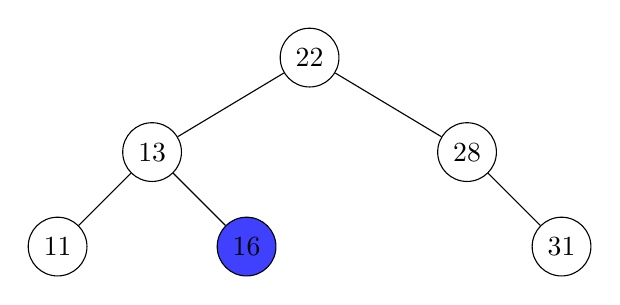
\begin{tikzpicture}[level distance =15mm,scale=0.8]
  \tikzstyle{level 1}=[sibling distance =5cm]
  \tikzstyle{level 2}=[sibling distance =3 cm]
  \tikzstyle{level 3}=[sibling distance =2 cm]
  \tikzstyle{every node}=[circle,draw]
  \node  {$22$}
  child {node{$13$}
          child {node{$11$}}
          child {node[fill=blue!75]{$16$}}
        }
  child {node {$28$}
         child [fill=none] {edge from parent[draw=none]}
         child {node{$31$}}
        };
\end{tikzpicture}
\caption{Suppression du nœud de clé 18 dans $a_0$}
\end{figure*}



Le cas d'un nœud interne $n$ est plus délicat : on se ramène au cas de la racine; il suffira de remplacer le sous--arbre dont $n$ est la racine par l'arbre allégé.


Pour ôter la racine d'un sous--arbre sans trop de modification on va choisir de le remplacer par un autre nœud de l'arbre. L'objectif est de minimiser le nombre de modifications : le nœud de clé maximale dans le fils gauche (ou de clé minimale dans le fils droit) est un bon choix car sa clé sépare les clés restantes. De plus ce nœud n'a pas de fils droit donc on le remplace facilement par son fils gauche.

On peut écrire les fonctions correspondantes
%-------------------------------------------------------------------------------
\begin{code}{Fonctions auxiliaires}
let rec maxArbre arbre = 
  match arbre with
  |Vide -> failwith "Arbre vide"
  |Noeud(g, r, Vide) -> r
  |Noeud(g, r, d) -> maxArbre d;;

let rec suppressionMax arbre = 
  match arbre with
  |Vide -> failwith "Arbre vide"
  |Noeud(g, r, Vide) -> g
  |Noeud(g, r, d) -> Noeud(g, r, suppressionMax d);;

let suppressionRacine arbre = 
  match arbre with
  |Vide -> Vide
  |Noeud(Vide, r, d) -> d
  |Noeud(g, r, d) ->  let y = maxArbre g in
                      Noeud(suppressionMax g, y, d);;
\end{code}
%-------------------------------------------------------------------------------
\begin{code}{Suppression d'un nœud}
let rec suppression k arbre = 
  match arbre with
  |Vide -> Vide
  |Noeud(g, r, d) when cle r = k 
                  -> suppressionRacine arbre
  |Noeud(g, r, d) when k < cle r 
                  -> Noeud((suppression k g), r, d)
  |Noeud(g, r, d) -> Noeud(g, r, (suppression k d));;
\end{code}
%-------------------------------------------------------------------------------
%-------------------------------------------------------------------------------
\begin{exo}{Fusion}{}
Écrire une fonction {\tt Fusion a b} qui joint deux 
arbres binaires de recherche ; on pourra utiliser les fonctions de coupure d'un arbre binaire de recherche.
%-------------------------------------------------------------------------------
\reponse
%-------------------------------------------------------------------------------
Si le premier arbre est non vide on coupe le second selon la racine du premier et on ajoute les morceaux aux deux fils.
%-------------------------------------------------------------------------------
\begin{ocaml}
let rec fusion arbre1 arbre2 =
  match arbre1 with
  |Vide -> arbre2
  |Noeud(g, r, d) -> let (pt, gd) = decoupage (cle r) arbre2 in
                      Noeud(fusion g pt, r, fusion d gd);;
\end{ocaml}
%-------------------------------------------------------------------------------
\end{exo}
%-------------------------------------------------------------------------------
%-------------------------------------------------------------------------------
\begin{figure*}]
\centering
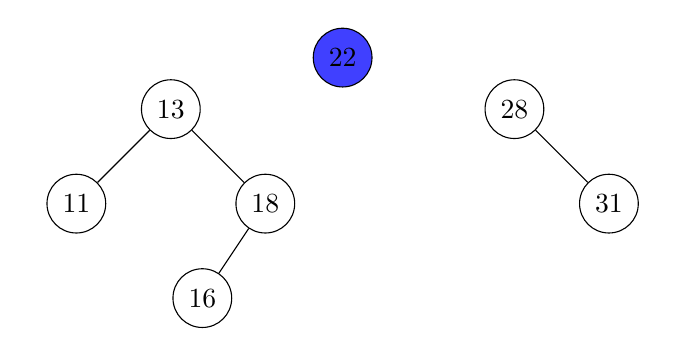
\begin{tikzpicture}[level distance =15mm,scale=0.8]
  \tikzstyle{level 1}=[sibling distance =10cm]
  \tikzstyle{level 2}=[sibling distance =3 cm]
  \tikzstyle{level 3}=[sibling distance =2 cm]
  \tikzstyle{every node}=[circle,draw]
  \node[fill=blue!75]{$22$}
  child {edge from parent[draw=none] node{$13$}
          child {node{$11$}}
          child {node{$18$}
                  child {node{$16$}}
                  child [fill=none] {edge from parent[draw=none]}
                 }
        }
  child {edge from parent[draw=none] node {$28$}
         child [fill=none] {edge from parent[draw=none]}
         child {node{$31$}}
        };
\end{tikzpicture}
\caption{Suppression de la racine dans $a_0$}
%-------------------------------------------------------------------------------
\bigskip
%-------------------------------------------------------------------------------
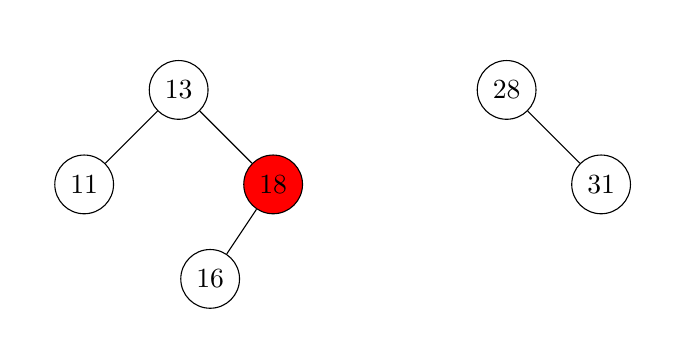
\begin{tikzpicture}[level distance =15mm,scale=0.8]
  \tikzstyle{level 1}=[sibling distance =10cm]
  \tikzstyle{level 2}=[sibling distance =3 cm]
  \tikzstyle{level 3}=[sibling distance =2 cm]
  \tikzstyle{every node}=[circle,draw]
  \node[draw = none]{}
  child {edge from parent[draw=none] node{$13$}
          child {node{$11$}}
          child {node[fill=red]{$18$}
                  child {node{$16$}}
                  child [fill=none] {edge from parent[draw=none]}
                 }
        }
  child {edge from parent[draw=none] node {$28$}
         child [fill=none] {edge from parent[draw=none]}
         child {node{$31$}}
        };
\end{tikzpicture}
\caption{Clé maximale du fils gauche}
%-------------------------------------------------------------------------------
\bigskip
%-------------------------------------------------------------------------------
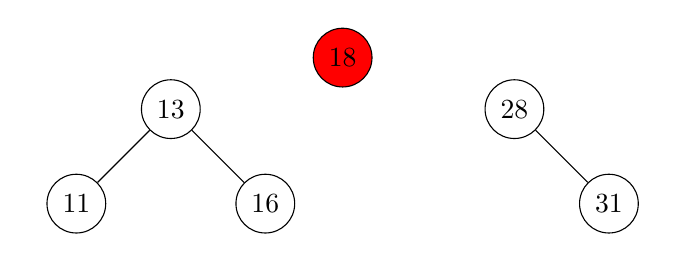
\begin{tikzpicture}[level distance =15mm,scale=0.8]
  \tikzstyle{level 1}=[sibling distance =10cm]
  \tikzstyle{level 2}=[sibling distance =3 cm]
  \tikzstyle{level 3}=[sibling distance =2 cm]
  \tikzstyle{every node}=[circle,draw]
  \node[fill=red]{18}
  child {edge from parent[draw=none] node{$13$}
          child {node{$11$}}
          child {node{$16$}}
        }
  child {edge from parent[draw=none] node {$28$}
         child [fill=none] {edge from parent[draw=none]}
         child {node{$31$}}
        };
\end{tikzpicture}
\caption{Déplacement du maximum}
%-------------------------------------------------------------------------------
\bigskip
%-------------------------------------------------------------------------------
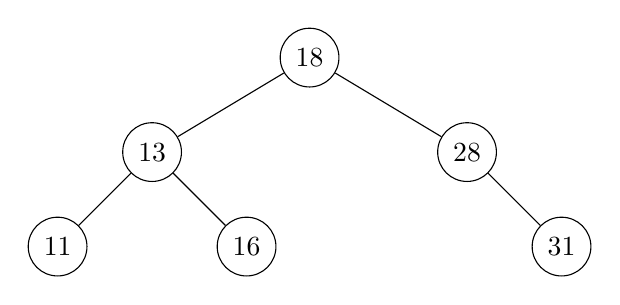
\begin{tikzpicture}[level distance =15mm,scale=0.8]
  \tikzstyle{level 1}=[sibling distance =5cm]
  \tikzstyle{level 2}=[sibling distance =3 cm]
  \tikzstyle{level 3}=[sibling distance =2 cm]
  \tikzstyle{every node}=[circle,draw]
  \node{18}
  child {node{$13$}
          child {node{$11$}}
          child {node{$16$}}
        }
  child {node {$28$}
         child [fill=none] {edge from parent[draw=none]}
         child {node{$31$}}
        };
\end{tikzpicture}
\caption{Arbre allégé}
\end{figure*}
%-------------------------------------------------------------------------------
\clearpage
%-------------------------------------------------------------------------------
\section{Application : dictionnaires}
%-------------------------------------------------------------------------------
%-------------------------------------------------------------------------------

Lors de l'étude des structures abstraites nous avons définis les dictionnaires (ou tableaux associatifs) qui sont des structures de données abstraites où l'on stocke des éléments munis d'une clé.

On travaillera donc  avec des éléments d'un type \type{'a * 'b} :

\begin{itemize}
    \item les premières composantes sont les {\bf clés}, leur type est muni d'une relation d'ordre total
    \item les secondes composantes sont d'un type quelconque.
\end{itemize}


L'implémentation du type abstrait doit définir :
%-------------------------------------------------------------------------------
\begin{itemize}
\item un type @'a * 'b dict@, on notera @'c@ le type @'a * 'b@,
\item une fonction @creerDict : 'a ->  'b -> 'c dict@, qui construit un dictionnaire vide, les variables passées en paramètre donnent un exemple d'élément qui pourrait être dans le dictionnaire,

\item une fonction @insertion : 'a -> 'b -> 'c dict -> unit@, qui insère un élément dans le dictionnaire,
\item une fonction @defini : 'a -> 'c dict -> bool@ qui teste si une clé correspond à une entrée,
\item une fonction @valeur : 'a -> 'c dict -> 'b@, qui retrouve, si elle existe, la valeur du dictionnaire associée à une clé,
\item une fonction @retrait : 'a -> 'c dict -> unit@, qui élimine un élément défini par sa clé, 
\end{itemize}
%-------------------------------------------------------------------------------
On remarquera que les fonctions ci-dessus correspondent à un type de données impératif : l'ajout ou le retrait d'un élément ne créent pas un nouveau dictionnaire.
%-------------------------------------------------------------------------------
%-------------------------------------------------------------------------------
\subsection{Implémentations déjà vues}
%-------------------------------------------------------------------------------
%-------------------------------------------------------------------------------
Nous avons déjà implémenté les dictionnaires à l'aide de listes d'associations, triées ou non triées? Les fonctions ne sont pas efficaces.

Nous avons utilisé des tables de hachages pour implémenter cette structure : les différentes fonctions sont alors très efficaces. Cependant il est difficile dans ce cas d'énumérer les éléments, ou d'utiliser la relation d'ordre des clés, par exemple pour déterminer les éléments dont les clés sont comprises entre deux bornes.
%-------------------------------------------------------------------------------
%-------------------------------------------------------------------------------
\subsection{Utilisation des arbres binaires de recherche}
%-------------------------------------------------------------------------------
%-------------------------------------------------------------------------------
Un arbre binaire de recherche permet de rechercher, ajouter ou enlever les éléments avec une complexité en ${\cal O}(h)$ où $h$ est la hauteur de l'arbre dont on peut espérer qu'elle soit de l'ordre de $\ln(n)$ où $n$ est la taille de l'arbre.

\begin{figure*}[ht]
\centering
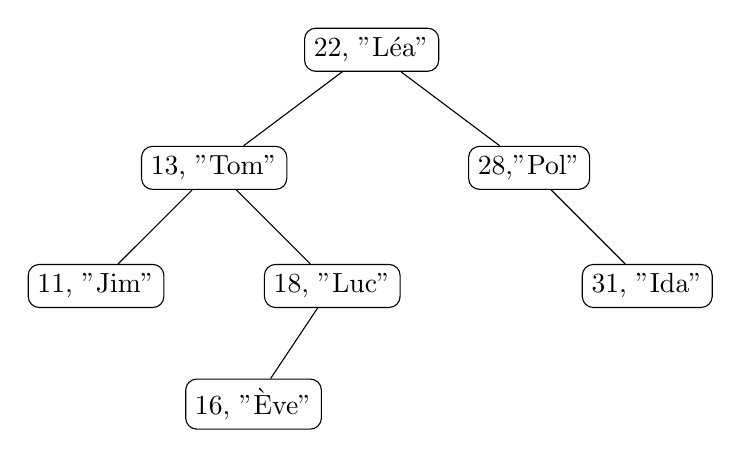
\begin{tikzpicture}[level distance =15mm]
  \tikzstyle{level 1}=[sibling distance =4cm]
  \tikzstyle{level 2}=[sibling distance =3cm]
  \tikzstyle{level 3}=[sibling distance =2cm]
  \tikzstyle{every node}=[rectangle,draw, rounded corners]
  \node {$22$, "Léa"}
  child {node{$13$, "Tom"}
          child {node{$11$, "Jim"}}
          child {node{$18$, "Luc"}
                  child {node{$16$, "Ève"}}
                  child [fill=none] {edge from parent[draw=none]}
                 }
        }
  child {node{$28$,"Pol"}
          child [fill=none] {edge from parent[draw=none]}
          child {node{$31$, "Ida"}}
        };
\end{tikzpicture}
\caption{Exemple de dictionnaire}
\end{figure*}

\newpage
Comme on veut un type non persistant qui utilise un type persistant, les arbres binaires, on doit encapsuler les arbres dans une structure ; ce peut être un enregistrement mutable ou, ce qui revient au même, une référence.

Les fonctions sont alors des adaptations.
%-------------------------------------------------------------------------------
\begin{code}{Implémentation de dictionnaires}
type 'a*'b dict = 'a * 'b abr ref;;

let cle = snd;;

let creerDict k v = ref Vide;;

let insertion k v dico =
    dico := insertionRacine (k, v) !dico;;
    
let defini k dico
  = chercher k !dico;;
   
let rec valeur k dico = 
  noeud k !dico;;

let retrait k dico = 
  dico := suppression k !dico;;
\end{code}
%-------------------------------------------------------------------------------
%-------------------------------------------------------------------------------
\begin{exo}{Implémentations d'ensembles}{}
Implémenter une structure d'ensemble mutable à l'aide d'arbres binaires de recherche : il faudra définir le 
type et les fonctions \type{ensembleVide, estVide, appartient, inserer, retirer}.

\reponse

La structure d'arbre n'est pas mutable : chaque fonction construit un nouvel arbre. Nous allons donc encapsuler un arbre, comme nous avons fait pour les files et les piles.

%-------------------------------------------------------------------------------
\begin{ocaml}
type 'a ensemble = {mutable contenu : 'a abr};;
\end{ocaml}
%-------------------------------------------------------------------------------

Les fonctions sont alors directement les traductions des fonctions sur les arbres.

%-------------------------------------------------------------------------------
\begin{ocaml}
let ensembleVide () = {contenu = Vide};;

let estVide ens = ens.contenu = Vide;;

let appartient x ens  = (chercher x ens.contenu);;

let inserer x ens  = 
 ens.contenu <- ajouterRacine x ens.contenu;;

let retirer x ens  = 
 ens.contenu <- suppression x ens.contenu;;
\end{ocaml}
\end{exo}
%-------------------------------------------------------------------------------
%-------------------------------------------------------------------------------
%-------------------------------------------------------------------------------
\section{Problème 1 : ancêtres commun}
%-------------------------------------------------------------------------------
%-------------------------------------------------------------------------------
%-------------------------------------------------------------------------------
Dans ce problème, on étudie les positions des éléments d'un arbre binaire de recherche.
%-------------------------------------------------------------------------------
%-------------------------------------------------------------------------------
\subsection{PPAC}
%-------------------------------------------------------------------------------
%-------------------------------------------------------------------------------
Un ancêtre commun de deux nœuds $n_1$ et $n_2$ d'un arbre est un nœud dont $n_1$ et $n_2$ sont descendants ; en particulier la racine est toujours un ancêtre commun de toute paire de nœuds.
%-------------------------------------------------------------------------------
%-------------------------------------------------------------------------------
\begin{question}{}{}
Montrer que, pour tout entier $h$, deux nœuds $n_1$ et $n_2$ admettent au plus un ancêtre commun à la profondeur $h$.
%-------------------------------------------------------------------------------
\reponse
%-------------------------------------------------------------------------------
Deux nœuds de même profondeur définissent deux sous-arbres disjoints : ils ne peuvent donc pas être en même temps ancêtres communs de $n_1$ et $n_2$.
\end{question}
%-------------------------------------------------------------------------------
%-------------------------------------------------------------------------------

Le {\sc Plus Proche Ancêtre Commun} (PPAC) de deux nœuds d'un arbre est l'ancêtre commun des deux nœuds de profondeur maximale. Son unicité découle de l'exercice précédent.
%-------------------------------------------------------------------------------
%-------------------------------------------------------------------------------
\begin{question}{}{}
Si $n_0$ est le PPAC de deux nœuds $n_1$ et $n_2$, prouver que les nœuds du chemin depuis la racine vers $n_0$ sont les ancêtres communs de $n_1$ et $n_2$
%-------------------------------------------------------------------------------
\reponse
%-------------------------------------------------------------------------------
Les ancêtres d'un d'un ancêtre commun sont des ancêtres communs, en particulier les ancêtres du PPAC sont des ancêtres communs. Comme il y a au plus un ancêtre commun pour un profondeur $h$, on a trouvé le seul ancêtre commun possible pour les profondeurs de 0 à celle, maximale, de $n_0$ donc pour toutes les profondeurs auxquelles il existe un ancêtre commun.
\end{question}
%-------------------------------------------------------------------------------
%-------------------------------------------------------------------------------
\subsection{PPAC dans un arbre binaire de recherche}
%-------------------------------------------------------------------------------
%-------------------------------------------------------------------------------
On suppose maintenant qu'on a affaire à un arbre binaire de recherche.

Deux nœuds $n_1$ et $n_2$ on des clés $k_1$ et $k-2$ telles que $k_1 < k_2$.
%-------------------------------------------------------------------------------
%-------------------------------------------------------------------------------
\begin{question}{}{ppac}
 Si $n$ est le PPAC $n_1$ et $n_2$, prouver qu'on a 
\begin{itemize}
\item soit $n = n_1$ et $n_2$ appartient au fils droit de $n_1$,
\item soit $n = n_2$ et $n_1$ appartient au fils gauche de $n_2$,
\item soit $n\ne n_1$, $n\ne n_2$, $n_1$ appartient au fils gauche de $n$ et $n_2$ appartient au fils droit de $n$.
\end{itemize}
%-------------------------------------------------------------------------------
\reponse
%-------------------------------------------------------------------------------
\begin{itemize}
\item Si $n = n_1$ alors $n_2$ est un descendant de $n_1$ de clé supérieure donc appartient au fils droit de $n_1$.
\item De même, si $n = n_2$, alors $n_1$ appartient au fils gauche de $n_2$,
\item Si $n$ est distinct de $n_1$ et $n_2$, alors $n_1$ et $n_2$ appartiennent aux fils de $n$. S'il appartenaient au même fils celui-ci serait un ancêtre commun, ce qui contredirait la maximalité de la profondeur. Ainsi $n_1$ et $n_2$ appartiennent à des fils distincts de $n$ ; l'ordre des clés impose alors que $n_1$ appartient au fils gauche de $n$ et $n_2$ appartient au fils droit de $n$.
\end{itemize}
\end{question}
%-------------------------------------------------------------------------------
%-------------------------------------------------------------------------------
\begin{question}{}{}
En déduire l'écriture d'une fonction qui permet de déterminer le PPAC des deux nœuds d'un A.B.R. à partir de leurs clés. On supposera, sans avoir besoin de le vérifier, que les deux clés sont bien les clés de nœuds de l'arbre.
%%-------------------------------------------------------------------------------
\reponse
\begin{ocaml}
let rec ppac arbre p q =
   (* On suppose p < q *)
    match arbre with
   |Vide -> failwith "Les elements ne sont pas dans l'arbre"
   |Noeud(g, n, d) when cle n < p -> ancetreCommun d p q
   |Noeud(g, n, d) when cle n > q -> ancetreCommun g p q
   |Noeud(g, n, d) -> n;;
\end{ocaml}
%-------------------------------------------------------------------------------
\end{question}
%-------------------------------------------------------------------------------
%-------------------------------------------------------------------------------
\subsection{Prédécesseur et successeur}
%-------------------------------------------------------------------------------
%-------------------------------------------------------------------------------
Le successeur (resp. prédécesseur) d'un nœud de clé $n$ est le nœud de l'arbre dont la clé suit (resp. précède) $n$ dans le parcours infixe. On remarquera que le successeur peut ne pas exister, dans le cas où la clé du nœud est maximale.
%-------------------------------------------------------------------------------
%-------------------------------------------------------------------------------
\begin{question}{}{}
On suppose que $a$ admet un prédécesseur $b$ dans un arbre binaire de recherche.

Montrer qu'on a 
\begin{itemize}
    \item soit $b$ est le nœud de clé maximale dans le fils gauche de $a$,
    \item soit $a$ est le nœud de clé minimale dans le fils droit de $b$.
\end{itemize}
%-------------------------------------------------------------------------------
\reponse
%-------------------------------------------------------------------------------
Si $c$ est le PPAC de $a$ et $b$, il n'est pas possible d'avoir $c\ne a$ et $c\ne b$ car sinon les clé de $b$ et de $a$ seraient séparées par la clé de $c$, ce qui contredit la définition du prédécesseur de $a$.

On est alors dans un des deux autres cas de la question \ref{ques:ppac} 
\end{question}
%-------------------------------------------------------------------------------
%-------------------------------------------------------------------------------
\begin{question}{}{}
Écrire deux fonctions qui calculent respectivement la clé minimale et la clé maximale dans un arbre binaire de recherche. 
%-------------------------------------------------------------------------------
\reponse
%-------------------------------------------------------------------------------
\begin{ocaml}
let rec minArbre arbre = 
   match arbre with
   |Vide -> failwith "Arbre vide"
   |Noeud(Vide, r, d) -> cle r
   |Noeud(g, r, d) -> minArbre g;;

let rec maxArbre arbre = 
   match arbre with
   |Vide -> failwith "Arbre vide"
   |Noeud(d, r, Vide) -> cle r
   |Noeud(g, r, d) -> maxArbre g;;
\end{ocaml}
\end{question}
%-------------------------------------------------------------------------------
%-------------------------------------------------------------------------------
\begin{question}{}{}
Écrire une fonction calculant la plus petite clé strictement supérieure à une valeur $k$ donnée dans un arbre binaire de recherche. %-------------------------------------------------------------------------------
\reponse
%-------------------------------------------------------------------------------
\begin{ocaml}
let rec suivant k arbre =
   match arbre with
   |Vide -> failwith "Les clé sont trop petites"
   |Noeud(g, r, d) when cle r = k  -> minArbre d
   |Noeud(g, r, d) when cle r < k -> suivant k d
   |Noeud(Vide, r, d) -> cle r
   |Noeud(g, r, d) when maxArbre g <= k -> cle r
   |Noeud(g, r, d) -> suivant k g;;
;;
\end{ocaml}
\end{question}
%-------------------------------------------------------------------------------
%-------------------------------------------------------------------------------
%-------------------------------------------------------------------------------
\section{Problème 2 : B-arbres }
%-------------------------------------------------------------------------------
%-------------------------------------------------------------------------------
%-------------------------------------------------------------------------------
La création de branches dans un arbre binaire de recherche est effectuée au niveau des feuilles lors de l’ajout de nouvelles valeurs sans possibilité de réorganisation de la structure de l’arbre si les valeurs sont mal réparties. Ceci peut conduire à la construction d’arbres fortement déséquilibrés. De plus, un nœud est nécessaire pour chaque valeur contenue dans l’arbre, ce qui conduit à une structure peu compacte qui demande un grand nombre d’accès en lecture à des positions différentes. Ces accès sont très coûteux lorsque l’arbre est stocké sur un disque pour implanter une base de données par exemple.

Pour réduire ces deux défauts, on modifie la structure des arbres binaires de recherche en associant un nombre de valeurs plus important au niveau de chaque nœud pour séparer les éléments.

L’objectif de ce problème est d’étudier une implantation particulière de cette structure les B-arbres d'ordre $t$.
%-------------------------------------------------------------------------------
\begin{defin}{Arbre d’ordre $t$ de nombres entiers}
Soit $t$ un nombre entier supérieur ou égal à 2, un B-Arbre d’ordre $t$ de nombres entiers $a$ est une structure récursive d'objets de 2 types.
\begin{itemize}
    \item Soit une feuille contenant une suite strictement croissante $(e_1, e_2, \ldots, e_p)$ d'entiers, les étiquettes, que l'on notera ${\cal E}(a)$. 
    \item Soit un nœud contenant une suite strictement croissante de taille $p$ d’étiquettes également notée ${\cal E}(a)$  et une suite ${\cal A}(a) = (a_0 , a_2, \ldots, a_p)$ de sous-arbres $a_i$ possédant la même structure de B-Arbre d’ordre $n$.
\end{itemize}
\end{defin}
%-------------------------------------------------------------------------------
\begin{defin}{Rang}
La longueur de ${\cal E}(a)$ est appelé rang de la feuille ou du nœud
\end{defin}
%-------------------------------------------------------------------------------
\begin{defin}{B-arbre d’ordre $t$ de nombres entiers}
%-------------------------------------------------------------------------------
Un B-arbre est un Arbre d’ordre $t$ de nombres entiers qui vérifie les conditions

\begin{description}
\item[Condition de croissance]  : pour tout $i\in \{1,2, \ldots, p\}$, les étiquettes contenues dans $a_{i-1}$ sont toutes strictement inférieures à $e_i$ et es étiquettes contenues dans $a_i$ sont toutes strictement supérieures à $e_i$.
\item[Condition de taille] : le rang $p$ de chaque feuille ou nœud doit vérifier $t-1 \le p\le 2t-2$ sauf pour la racine pour laquelle la seule condition est $p\le 2t-2$.
\item[Condition d'équilibre] : toutes les feuilles sont à la même profondeur.
\end{description}
\end{defin}
%-------------------------------------------------------------------------------
\begin{figure*}[ht]
\centering
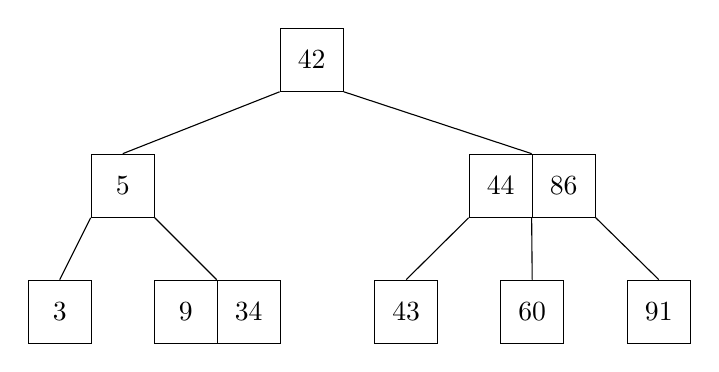
\begin{tikzpicture}[scale = 0.8,every node/.style={minimum size=0.8cm}]
\node[draw] (e0) at (5, 0) {42};
\node[draw] (e10) at (2, -2) {5};
\node[draw] (e11a) at (8, -2) {44};
\node[draw] (e11b) at (9, -2) {86};
\node[draw] (e20) at (1, -4) {3};
\node[draw] (e21a) at (3, -4) {9};
\node[draw] (e21b) at (4, -4) {34};
\node[draw] (e22) at (6.5, -4) {43};
\node[draw] (e23) at (8.5, -4) {60};
\node[draw] (e24) at (10.51, -4) {91};
\draw (e0.south west) -- (e10.north);
\draw (e0.south east) -- (e11b.north west);
\draw (e10.south west) -- (e20.north);
\draw (e10.south east) -- (e21b.north west);
\draw (e11a.south west) -- (e22.north);
\draw (e11b.south west) -- (e23.north);
\draw (e11b.south east) -- (e24.north);
\end{tikzpicture}
\caption{B-arbre d'ordre 2}
\label{Barbre}
\end{figure*}
%-------------------------------------------------------------------------------
{\bf Remarques}

\begin{itemize}
\item La condition de taille impose qu'on a $t\ge 2$. 

\item Une feuille qui n'est pas à la racine n'est jamais vide car $t-1\ge 1$.

\item Pour $t=2$, un nœud ou une feuille admet 1 ou 2 étiquettes donc un nœud admet 2 ou 3 fils ; on parle dans ce cas d'arbre 2-3.

\item Un nœud ou une feuille de rang $p$ d’un B-Arbre d’ordre $t$ est {\bf complet} si et seulement si $p  = 2t-2$.
\item La condition d'équilibre impose un arbre équilibré.
\end{itemize}
%-------------------------------------------------------------------------------
%-------------------------------------------------------------------------------
\begin{question}{}{}
Donner des bornes de la taille d'un B-arbre d'ordre $t$ en fonction de $t$ et de la hauteur.
%-------------------------------------------------------------------------------
\reponse
%-------------------------------------------------------------------------------
$t^h \le n \le (2t-1)^{h-1}(2t-2)$
\end{question}
%-------------------------------------------------------------------------------
%-------------------------------------------------------------------------------
{\bf Formalisation}
%-------------------------------------------------------------------------------
\begin{itemize}
    \item L’ensemble des feuilles de l’arbre $a$ est noté ${\cal F}(a)$. 

    \item L’ensemble des nœuds de l’arbre $a$ est noté ${\cal N}(a)$.

    \item L’ensemble des étiquettes de l’arbre $a$ est noté ${\cal C}(a)$.
\end{itemize}

Les étiquettes des nœuds d’un B-Arbre vérifient donc la contrainte suivante :

pour $b\in {\cal N}(a)$ avec ${\cal E}(b) = (e_1 , e_2, \ldots, e_{p})$ et ${\cal A}(b) = (b_0 , b_1, \ldots, b_p)$,
\[\left\{\begin{matrix}
&\forall v \in {\cal C}(b_0)& v < e_1\\
\forall i\in \{1, 2, \ldots, p-1\}& \forall v\in {\cal C}(b_i)& e_{i-1} < v < e_i\\
&\forall v\in {\cal C}(b_p)& e_p  < v
\end{matrix}\right.\]
%-------------------------------------------------------------------------------
\subsubsection{Inplémentation OCaml}
%-------------------------------------------------------------------------------
Un B-Arbre d’entiers est représenté par la constante globale  \type{t} et le type suivant.
%-------------------------------------------------------------------------------
\begin{ocaml}
type bArbre = |Feuille of int * int list
              |Noeud of int * int list * bArbre list;;
\end{ocaml}
%-------------------------------------------------------------------------------
Dans \type{Noeud(p, e, f)}, \type{p} est le rang du nœud, \type{e} est la liste strictement croissante  des étiquettes et \type{f} est la liste des fils dans l'ordre de valeurs croissantes et séparées par les étiquettes. 

Dans \type{Feuille(p, liste)}, \type{p} est le rang du nœud, \type{e} est la liste strictement croissante  des étiquettes.

\type{p} est donc la longueur de \type{e} et, pour les nœuds, \type{f} est de longueur \type{p+1}

L'exemple ci-dessus correspond à
%-------------------------------------------------------------------------------
\begin{ocaml}
let t = 2;;
let a = Noeud(1, 
              [42],
              [Noeud(1, 
                     [5],
                     [Feuille(1, [23]); Feuille(2, [9; 34])]
                    );
               Noeud(2,
                     [44; 86],
                     [Feuille(1, [43]);
                      Feuille(1, [60]);
                      Feuille(1, [91])]
                     )]);;
\end{ocaml}
%-------------------------------------------------------------------------------
%-------------------------------------------------------------------------------
\subsection{Premières fonctions}
%-------------------------------------------------------------------------------
%-------------------------------------------------------------------------------
\begin{question}{Calcul du nombre de valeurs}{}
Écrire une fonction \type{taille : bArbre -> bool} qui renvoie le nombre d’étiquettes entières contenues dans le B-Arbre a, c’est-à-dire le cardinal de ${\cal C}(a)$. 

L’algorithme utilisé ne devra parcourir qu’une seule fois l’arbre
%-------------------------------------------------------------------------------
\reponse
%-------------------------------------------------------------------------------
La fonction doit utiliser une fonction qui calcule la somme des cardinaux des étiquettes dans la liste des couples.

On peut définir une fonction auxiliaire
\begin{ocaml}
let rec taille a =
   let rec taille_fils liste =
      match liste with
      |[] -> 0
      |b::reste -> taille b + (taille_fils reste) in
   match a with
   |Feuille(p, e) -> p 
   |Noeud(p, e, f) -> p + taille_fils f;;  
\end{ocaml}

On peut considérer les deux fonctions au même plan avec une récursivité croisée
\begin{ocaml}
let rec taille a =
   match a with
   |Feuille(p, e) -> p 
   |Noeud(p, e, f) -> p + taille_fils f
and taille_fils liste =
    match liste with
    |[] -> 0
    |b::reste -> taille b + (taille_fils reste);;
\end{ocaml}

C'est dans ce contexte que les fonctions d'itérations peuvent être utile
\begin{ocaml}
let rec taille a =
   match a with
   |Feuille(p, e) -> p 
   |Noeud(p, e, f) -> let fn b s = taille b + s in 
                      p + List.fold_right fn f 0;;
\end{ocaml}

\begin{ocaml}
let rec taille a =
   match a with
   |Feuille(p, e) -> p 
   |Noeud(p, e, f) -> let fn s b = taille b + s in
                      p + List.fold_left fn 0 f;;
\end{ocaml}
Gagne-t-on en lisibilité ?
\end{question}
%-------------------------------------------------------------------------------
%-------------------------------------------------------------------------------
\begin{question}{Recherche d’une étiquette}{}
Écrire une fonction \type{recherche : int -> bArbre -> bool} telle que \type{recherche k arbre} sur un B-Arbre \type{arbre} renvoie la valeur \type{true} si et seulement si $k$ appartient à ${\cal C}(\texttt{arbre})$.
%-------------------------------------------------------------------------------
\reponse
%-------------------------------------------------------------------------------
On commence par l'appartenance à une liste
\begin{ocaml}
let rec appartient k liste = 
   match liste with
   |[] -> false
   |t::q -> k = t || appartient k q;;
\end{ocaml}

\begin{ocaml}
let rec recherche k arbre =
   match arbre with
   |Feuille(p, e) -> appartient k e
   |Noeud(p, te::qe, tf::qf) when k < te -> recherche k tf
   |Noeud(p, te::qe, tf::qf) -> recherche (Noeud(p-1, qe, qf))
   |Noeud(p, [], tf::qf) -> recherche k tf
   |_ -> failwith "Ceci ne devrait pas arriver";;
\end{ocaml}
\end{question}
%-------------------------------------------------------------------------------
%-------------------------------------------------------------------------------
\subsection{Insertion sans condition de taille}
%-------------------------------------------------------------------------------
%-------------------------------------------------------------------------------
L’ajout d’une valeur dans un B-Arbre consiste à parcourir l’arbre de la racine vers la feuille qui devra contenir la valeur en suivant le même algorithme que pour rechercher une valeur. Lorsque l'on parvient à une feuille, on ajoute la valeur dans la liste des étiquettes.
%-------------------------------------------------------------------------------
%-------------------------------------------------------------------------------
\begin{question}{}{}
Dessiner l'arbre obtenu en ajoutant 73 à l'exemple de la figure \ref{Barbre}.
%-------------------------------------------------------------------------------
\reponse
%-------------------------------------------------------------------------------
\[
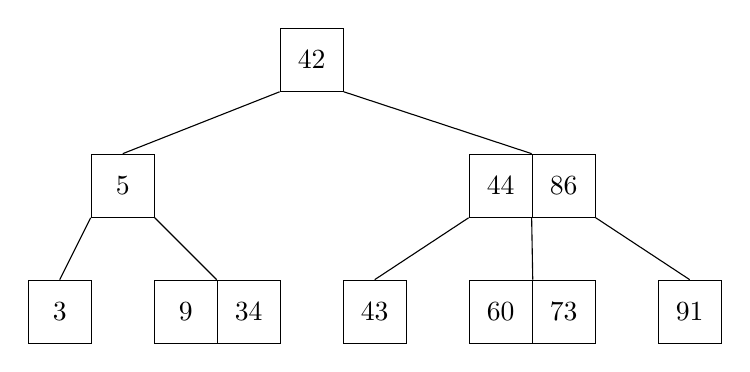
\begin{tikzpicture}[scale = 0.8,every node/.style={minimum size=0.8cm}]
\node[draw] (e0) at (5, 0) {42};
\node[draw] (e10) at (2, -2) {5};
\node[draw] (e11a) at (8, -2) {44};
\node[draw] (e11b) at (9, -2) {86};
\node[draw] (e20) at (1, -4) {3};
\node[draw] (e21a) at (3, -4) {9};
\node[draw] (e21b) at (4, -4) {34};
\node[draw] (e22) at (6, -4) {43};
\node[draw] (e23a) at (8, -4) {60};
\node[draw] (e23b) at (9, -4) {73};
\node[draw] (e24) at (11, -4) {91};
\draw (e0.south west) -- (e10.north);
\draw (e0.south east) -- (e11b.north west);
\draw (e10.south west) -- (e20.north);
\draw (e10.south east) -- (e21b.north west);
\draw (e11a.south west) -- (e22.north);
\draw (e11b.south west) -- (e23a.north east);
\draw (e11b.south east) -- (e24.north);
\end{tikzpicture}
\]
\end{question}
%-------------------------------------------------------------------------------
%-------------------------------------------------------------------------------
\begin{question}{}{}
Écrire une fonction \type{inserer : int -> int list -> int list} qui insère un élément dans une liste triée afin d'obtenir une liste toujours triée.

On pourra supposer que la valeur à insérer n'est pas dans la liste.
%-------------------------------------------------------------------------------
\reponse
%-------------------------------------------------------------------------------
\begin{ocaml}
let rec inserer k liste =
   match liste with
   |[] -> [k]
   |t::q when k < t -> k :: liste
   |t::q -> t :: (inserer k q);;
\end{ocaml}
\end{question}
%-------------------------------------------------------------------------------
%-------------------------------------------------------------------------------
\begin{question}{}{}
Écrire une fonction \type{position : int -> int list -> int} telle que \type{position k e} où \type{e} est une liste représentant une suite strictement croissante d'étiquettes $(e_1, e_2, \ldots, e_p)$ renvoie l'entier $i$ tel que
\begin{itemize}
    \item $i=0$ si on a $k < e_1$,
    \item $i=p$ si on a $k > e_p$,
    \item $i$ est l'unique entier tel que $e_i < k < e_{i+1}$ sinon.
\end{itemize}
On supposera que $k$ n'est pas un élément de \type{e}.
%-------------------------------------------------------------------------------
\reponse
%-------------------------------------------------------------------------------
\begin{ocaml}
let rec position k liste =
   match liste with
   |t::q when k < t -> 0
   |[t] -> 1
   |t1::t2::q when k < t2 -> 1
   |t::q  -> 1 + position k q
   |[] -> failwith "Ceci ne devrait pas arriver";;
\end{ocaml}
\end{question}
%-------------------------------------------------------------------------------
%-------------------------------------------------------------------------------
\begin{question}{}{}
Écrire une fonction \type{ajouter : int -> bArbre -> bArbre} qui ajoute un élément dans sa feuille. On supposera que cet élément n'est pas dans l'arbre.
%-------------------------------------------------------------------------------
\reponse
%-------------------------------------------------------------------------------
\begin{ocaml}
let rec ajouter k arbre =
   match arbre with
   |Feuille(p, e) -> Feuille(p+1, inserer k e)
   |Noeud(p, e, f) -> let i = position k e in
                      let rec changer pos liste = 
                         match pos, liste with
                         |0, t::q -> (ajouter k t) :: q
                         |i, t::q -> t :: (changer (pos - 1) q)
                         |_ -> failwith "Erreur dans les fils" in
                      Noeud(p, e, changer i f);;
\end{ocaml}
\end{question}
%-------------------------------------------------------------------------------
%-------------------------------------------------------------------------------
\subsection{Dépassement du rang}
%-------------------------------------------------------------------------------
%-------------------------------------------------------------------------------
Si la feuille dans laquelle on insère la valeur lors d'une insertion était complète, l'ordre devient trop grand: il vaut maintenant $2t-1$. 

On sépare alors les étiquettes en 3 :

\begin{itemize}
    \item les $t-1$ premières étiquettes forment une feuille $f_1$,
    \item les $t-1$ dernières  forment une feuille $f_2$,
    \item l'étiquette centrale, qui sépare ces deux feuilles, est notée $e'$.
\end{itemize}

Si la feuille était le fils $a_i$ d'un nœud,  on remplace la suite de fils et d'étiquettes 

$a_0, e_1, a_1, \ldots, e_{i-1}, a_i, e_i, a_{p-1}, e_p, a_p$ par 
$a_0, e_1, a_1, \ldots, e_{i-1}, f_1, e', f_2, e_i, a_{p-1}, e_p, a_p$
%-------------------------------------------------------------------------------
%-------------------------------------------------------------------------------
\begin{question}{}{}
Dessiner l'arbre obtenu en ajoutant 73 puis 37 à l'exemple de la figure \ref{Barbre}.
%-------------------------------------------------------------------------------
\reponse
%-------------------------------------------------------------------------------
\[
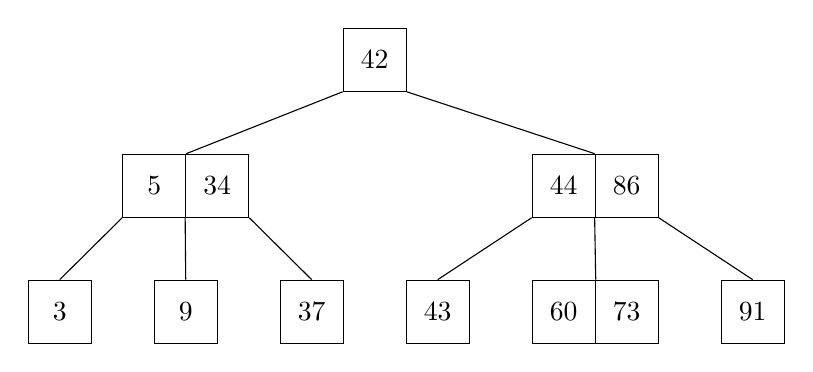
\begin{tikzpicture}[scale = 0.8,every node/.style={minimum size=0.8cm}]
\node[draw] (e0) at (5, 0) {42};
\node[draw] (e10a) at (1.5, -2) {5};
\node[draw] (e10b) at (2.5, -2) {34};
\node[draw] (e11a) at (8, -2) {44};
\node[draw] (e11b) at (9, -2) {86};
\node[draw] (e20) at (0, -4) {3};
\node[draw] (e21) at (2, -4) {9};
\node[draw] (e21n) at (4, -4) {37};
\node[draw] (e22) at (6, -4) {43};
\node[draw] (e23a) at (8, -4) {60};
\node[draw] (e23b) at (9, -4) {73};
\node[draw] (e24) at (11, -4) {91};
\draw (e0.south west) -- (e10a.north east);
\draw (e0.south east) -- (e11b.north west);
\draw (e10a.south west) -- (e20.north);
\draw (e10b.south west) -- (e21.north);
\draw (e10b.south east) -- (e21n.north);
\draw (e11a.south west) -- (e22.north);
\draw (e11b.south west) -- (e23a.north east);
\draw (e11b.south east) -- (e24.north);
\end{tikzpicture}
\]
\end{question}
%-------------------------------------------------------------------------------
%-------------------------------------------------------------------------------
Après cette scission d'une feuille, on ajoute une étiquette dans son nœud père mais, si celui-ci est complet, il a une étiquette de trop et il faut aussi le séparer et ajouter une étiquette au niveau du dessus. Ce procédé peut se poursuivre.
%-------------------------------------------------------------------------------
%-------------------------------------------------------------------------------
\begin{question}{}{}
Dessiner l'arbre obtenu en ajoutant 73 puis 37 puis 68 à l'exemple de la figure \ref{Barbre}.
%-------------------------------------------------------------------------------
\reponse
%-------------------------------------------------------------------------------
\[
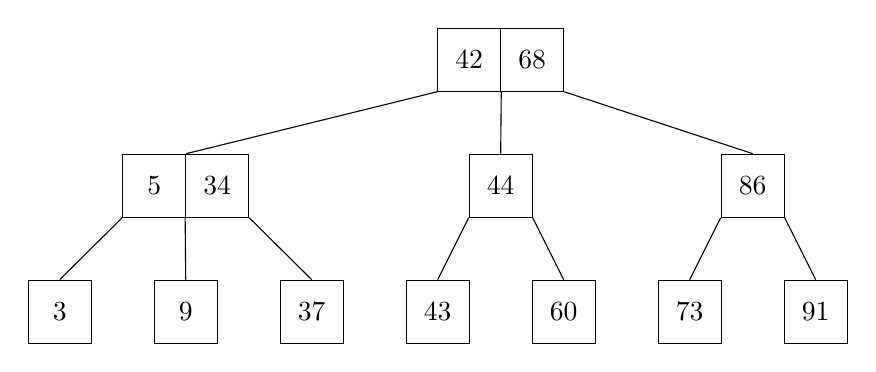
\begin{tikzpicture}[scale = 0.8,every node/.style={minimum size=0.8cm}]
\node[draw] (e0) at (6.5, 0) {42};
\node[draw] (e1) at (7.5, 0) {68};
\node[draw] (e10a) at (1.5, -2) {5};
\node[draw] (e10b) at (2.5, -2) {34};
\node[draw] (e12) at (7, -2) {44};
\node[draw] (e13) at (11, -2) {86};
\node[draw] (e20) at (0, -4) {3};
\node[draw] (e21) at (2, -4) {9};
\node[draw] (e21n) at (4, -4) {37};
\node[draw] (e22) at (6, -4) {43};
\node[draw] (e23a) at (8, -4) {60};
\node[draw] (e23b) at (10, -4) {73};
\node[draw] (e24) at (12, -4) {91};
\draw (e0.south west) -- (e10a.north east);
\draw (e0.south east) -- (e12.north);
\draw (e1.south east) -- (e13.north);
\draw (e10a.south west) -- (e20.north);
\draw (e10b.south west) -- (e21.north);
\draw (e10b.south east) -- (e21n.north);
\draw (e12.south west) -- (e22.north);
\draw (e12.south east) -- (e23a.north);
\draw (e13.south west) -- (e23b.north);
\draw (e13.south east) -- (e24.north);
\end{tikzpicture}
\]
\end{question}
%-------------------------------------------------------------------------------
%-------------------------------------------------------------------------------
Lorsqu'un nœud complet (ou une feuille complète) d'un B-arbre d'ordre $t$ reçoit une étiquette de plus il n'est plus un B-arbre d'ordre $t$, on le découpe. Si la suite de ses étiquettes et fils est $a_0, e_1, a_1, e_2, \ldots, a_{2t-2}, e_{2t-1}, a_{2t-1}$, on crée deux nœuds et une étiquette :
\begin{itemize}
    \item un nœud $g$ de rang $t-1$ associé à $a_0, e_1, a_1, e_2, \ldots, a_{t-2}, e_{t-1}, a_{t-1}$,
    \item un nœud $d$ de rang $t-1$ associé à $a_t, e_{t+1}, a_{t+1}, e_{t+2}, \ldots, a_{2t-2}, e_{2t-1}, a_{2t-1}$,
    \item une étiquette $e=e_t$.
\end{itemize}

Dans le cas d'une feuille, $g$ et $d$ sont des feuilles.
%-------------------------------------------------------------------------------
%-------------------------------------------------------------------------------
\begin{question}{}{}
Écrire une fonction \type{decoupage : int -> 'a list -> ('a list * 'a * 'a list)} telle que \type{decoupage k liste} appliquée à une liste $[x_0;x_1;\cdots;x_{n-1}]$ avec $n> k$ renvoie le triplet
$\bigl([x_0;x_1;\cdots;x_{k-1}], x_k, [x_{k+1};\cdots;x_{n-1}]\bigr)$
%-------------------------------------------------------------------------------
\reponse
%-------------------------------------------------------------------------------
\begin{ocaml}
let rec decoupage k liste =
   match k, liste with
   |0, t::q -> [], t, q
   |k, t::q -> let g, x, d = decoupage (k-1) q in t::g, x, d
   |k, [] -> failwith "Liste trop petite";;
\end{ocaml}
\end{question}
%-------------------------------------------------------------------------------
%-------------------------------------------------------------------------------
\begin{question}{}{}
Écrire une fonction \type{scission : bArbre -> (bArbre * int * bArbre)}
telle que \type{scissionBArbre a} appliquée à un B-Arbre d’ordre $t$ dont la racine est de rang $2t-1$  renvoie le triplet $(g, e, d)$ défini ci-dessus.
%-------------------------------------------------------------------------------
\reponse
%-------------------------------------------------------------------------------
\begin{ocaml}
let scission arbre =
   let r = t - 1 in
   match arbre with
   |Feuille(p, e) -> let eg, e, ed = decoupage r e in
                     Feuille(r, eg), e, Feuille(r, ed)
   |Noeud(p, e, f) -> let g, x, d = decoupage r e in
                      let a, y, b = decoupage t f in
                      Noeud(r, g, a), x, Noeud(r, d, y::b);;
\end{ocaml}
\end{question}
%-------------------------------------------------------------------------------
%-------------------------------------------------------------------------------
Pour écrire la fonction d'insertion, on va utiliser un nouveau type pour le résultat d'une fonction auxiliaire d'insertion :
\begin{ocaml}
type insert = Bon of bArbre | Split of bArbre * int * bArbre;;
\end{ocaml}
Si l'insertion au niveau considéré n'a pas donné lieu à une scission, on renvoie simplement un arbre, si l'insertion impose une scission on renvoie les 3 composantes de la scission.
%-------------------------------------------------------------------------------
%-------------------------------------------------------------------------------
\begin{question}{}{}
Modifier la fonction \type{ajouter} en tenant compte des modifications données ci-dessus.
%-------------------------------------------------------------------------------
\reponse
%-------------------------------------------------------------------------------
On va soit changer un arbre par un autre ou par deux autres dans la liste des fils.

L'élément d'indice $i$ (le fils à changer) est obtenu par

\begin{ocaml}
let rec ieme i liste =
   match i, liste with
   |0, t::q -> t
   |i, t::q -> ieme (i-1) q
   |i, [] -> failwith "Liste trop courte";;
\end{ocaml}

Changer un élément à l'indice $i$ par $x$ se fait par
\begin{ocaml}
let rec changer i x liste =  
   match i, liste with
   |0, t::q -> x::q
   |i, t::q -> t::(changer (i-1) x q)
   |i, [] -> failwith "Liste trop courte";;
\end{ocaml}

Changer un élément à l'indice $i$ par $x$ et $y$ se fait par
\begin{ocaml}
let rec changer2 i x y liste =  
   match i, liste with
   |0, t::q -> x::y::q
   |i, t::q -> t::(changer2 (i-1) x y q)
   |i, [] -> failwith "Liste trop courte";;
\end{ocaml}

Le rang est calculé par 
\begin{ocaml}
let rang arbre = 
   match arbre with
   |Feuille(p, e) -> p
   |Noeud(p, e, f) -> p;;
\end{ocaml}

Le découpage possible d'un arbre est donné par 
\begin{ocaml}
let sortie arbre = 
   if rang arbre < 2*t -1
   then Bon arbre
   else Split (scission arbre);;
\end{ocaml}

On crée la sortie de type insert :
\begin{ocaml}
let rec add k arbre =
   match arbre with
   |Feuille(p, e) -> Sortie (Feuille(p+1, inserer k e))
   |Noeud(p, e, f) 
      -> let pos = position k e in
         match add k (ieme pos f) with
         |Bon a -> Bon (Noeud(p, e, changer pos a f))
         |Split(g, x, d) -> Sortie (Noeud(p+1, 
                                          inserer x e, 
                                          changer2 pos g d f));;
\end{ocaml}

On peut alors écrire
\begin{ocaml}
let ajouter k arbre =
   match add k arbre with
   |Bon a -> a
   |Split(g, x, d) -> Noeud(1, [x], [g; d]);;
\end{ocaml}
\end{question}
%-------------------------------------------------------------------------------
%-------------------------------------------------------------------------------
\begin{question}{}{}
Écrire une fonction \type{construire\_arbre : int list -> bArbre} qui construit un arbre contenant les élément de la liste. 
%-------------------------------------------------------------------------------
\reponse
%-------------------------------------------------------------------------------
\begin{ocaml}
let faire liste = 
   List.fold_right ajouter liste (Feuille(0, []));;
\end{ocaml}
\end{question}
%-------------------------------------------------------------------------------
%-------------------------------------------------------------------------------
